\documentclass[14pt]{extarticle}

\usepackage{projectstemplate}
\usepackage[askip=3mm, bskip=3mm]{terminal}
\usepackage[askip=3mm, bskip=3mm]{mylisting}
\usepackage{tikz}
\usepackage{terminal}
\usetikzlibrary{positioning, shapes.geometric}

\title{Задание проекта \\ "Baremetal шифрование обмена"}

\begin{document}

\maketitle

\tableofcontents

\clearpage

\section{Термины и определения}

\begin{itemize}

 \item \textbf{Открытый текст} --- массив данных с секретной информацией\footnotemark{}.

  \footnotetext{\url{https://en.wikipedia.org/wiki/Plaintext}}

 \item \textbf{Шифротекст} --- шифрованный открытый текст\footnotemark{}.

  \footnotetext{\url{https://en.wikipedia.org/wiki/Plaintext}}

 \item \textbf{Алгоритм шифрования} --- алгоритм преобразования открытого текста
  в шифротекст и наоборот\footnotemark{}.
  Алгоритм шифрования всегда известен и не считается секретной информацией.

  \footnotetext{\url{https://en.wikipedia.org/wiki/Encryption}}

 \item \textbf{Ключ шифрования} --- массив данных, необходимый для алгоритма
  шифрования\footnotemark{}.
  Он обеспечивает уникальность шифрования, т.е. один и тот же алгоритм, получивший
  на вход один и тот же открытый текст, но разные ключи, даст разные шифротексты.
  В общем случае для шифрования и расшифрования используются разные ключи.
  Ключ, необходимый для расшифрования шифротекста в открытый текст, является секретным.
  Получивший его злоумышленник может восстановить открытый текст по имеющемуся
  в открытом доступен шифротексту.

  \footnotetext{\url{https://en.wikipedia.org/wiki/Key_(cryptography)}}

 \item \textbf{Симметричный алгоритм шифрования} --- алгоритм шифрования,
  использующий один и тот же ключ как для шифрования, так и для расшифрования.
  Работает быстрее асимметричных алгоритмов, но является менее надежным.
  Cемейство алгоритмов AES\footnotemark{} является самым распространенным примером симметричных
  алгоритмов.

  \footnotetext{\url{https://en.wikipedia.org/wiki/Advanced_Encryption_Standard}}
  
 \item \textbf{Вектор инициализации} --- массив данных, использующийся для шифрования
  вместе с ключом в алгоритме шифрования\footnotemark{}.
  Обычно уникален для каждой сессии шифрования и расшифрования.
  Его отличие от ключа в том, что он имеет меньший размер и подходит для передачи
  вместе с зашифрованным сообщением.
  Обычно не является секретным.
  Нужен для того, чтобы для одного и того же открытого текста, зашифрованного одним и тем
  же ключом, получался разный шифротекст.
  Это повышает устойчивость шифрования к взлому.

  \footnotetext{\url{https://en.wikipedia.org/wiki/Initialization_vector}}

\end{itemize}

\section{Задание}

\subsection{Общие сведения о системе}

Это задание предлагает для разработки систему, которую можно проиллюстрировать
схемой на рис.~\ref{fig:scheme}.

\begin{figure}[h!]
 \centering
 \begin{tikzpicture}[
  box/.style={draw, minimum width=3.5cm, minimum height=5cm},
  font=\small
 ]

  % ПК блок
  \node[box] (pc) {};
  \node[above=0.2cm of pc] {ПК};
  \node[anchor=north, inner sep=0pt] at ([yshift=-0.5cm]pc.north) 
   {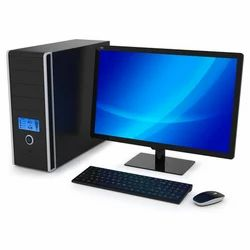
\includegraphics[width=1.5cm]{pc.jpg}};
  \node[anchor=north, inner sep=0pt] (pckey) at ([yshift=2.5cm]pc.south) 
   {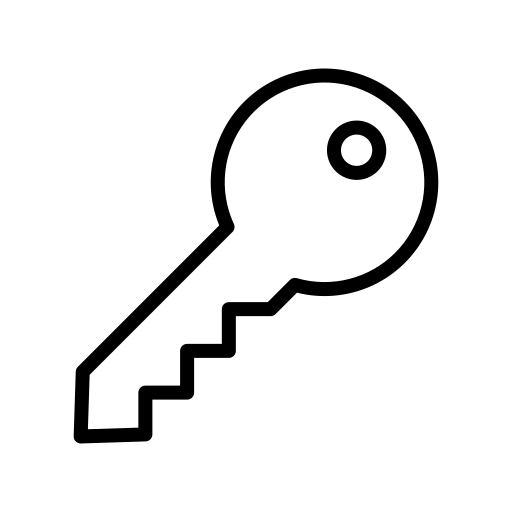
\includegraphics[width=1.0cm]{key.png}};
  \node[align=center, below=0.1cm of pckey] {Ключ\\шифрования};

  % Контроллер блок
  \node[box, right=3cm of pc] (ctrl) {};
  \node[above=0.2cm of ctrl] {Контроллер};
  \node[anchor=north, inner sep=0pt] at ([yshift=-0.5cm]ctrl.north) 
   {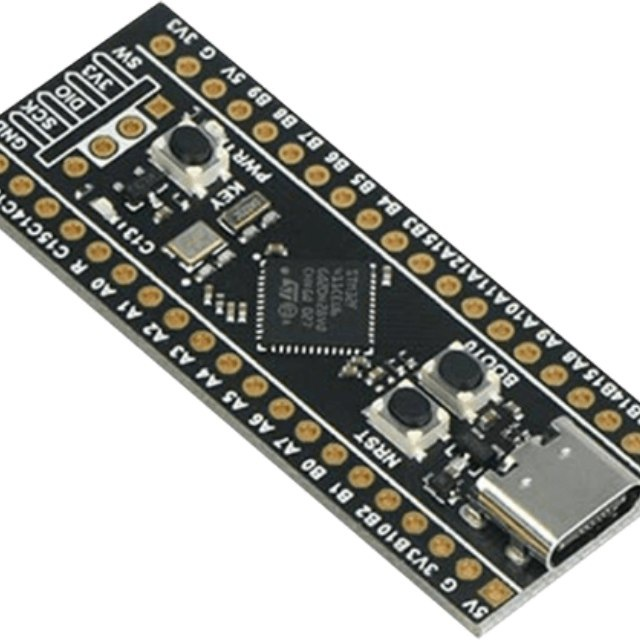
\includegraphics[width=1.5cm]{blackpill.jpg}};
  \node[anchor=north, inner sep=0pt] (ctrlkey) at ([yshift=2.5cm]ctrl.south) 
   {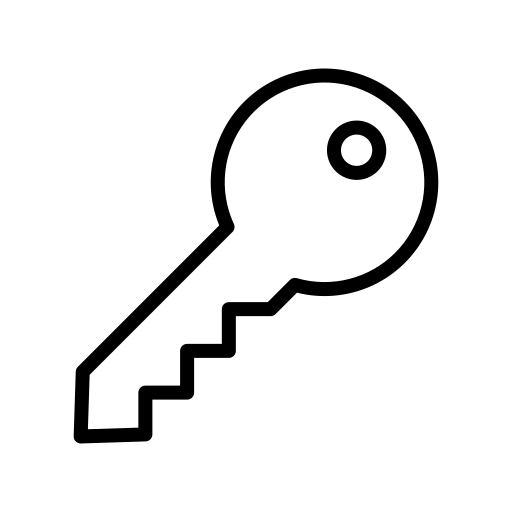
\includegraphics[width=1.0cm]{key.png}};
  \node[align=center, below=0.1cm of ctrlkey] {Ключ\\шифрования};

  % Соединение USB
  \draw[-] (pc.east) -- (ctrl.west) node[midway, above] {USB};
  \fill (pc.east) circle (2pt);
  \fill (ctrl.west) circle (2pt);
 \end{tikzpicture}
 \caption{Схема системы}\label{fig:scheme}
\end{figure}

Компоненты системы:

\begin{itemize}

 \item \textbf{Контроллер} --- устройство STM32F411CEU6 (WeAct BlackPill 2.0).
  Во время конфигурации после первого запуска сохраняет ключ шифрования в
  энергонезависимой (Flash) памяти устройства.
  Далее использует этот ключ для расшифрования входящих шифротекстов и шифрования
  исходящих открытых текстов.

 \item \textbf{ПК} --- персональный компьютер, выполняющий конфигурацию контроллера
  и обменивающийся с ним шифротекстом.
  Пользователь ПК создает ключ шифрования и устанавливает его на контроллер.
  После этого с помощью ключа шифруются исходящие открытые тексты и расшифровываются
  входящие шифротексты.

 \item \textbf{USB} --- среда обмена между ПК и контроллером.
  По USB ПК устанавливает ключ на контроллер.
  После этого USB становится защищенным каналом связи, по которому передаются
  только шифротексты.

 \item \textbf{Ключ шифрования} --- ключ шифрования симметричного алгоритма.
  Генерируется на ПК и устанавливается на контроллер при его первом после
  перепрошивки запуске.

\end{itemize}

\subsection{Функциональные требования}

\begin{enumerate}

 \item После установки образа ПО контроллер должен переходить в состояние
  ``Конфигурирование''.
  В этом состоянии он ожидает установку ключа шифрования от ПК по USB.
  После приема сообщения с ключом контроллер должен отправлять по USB признак
  ``успешно'', если ключ из входящего сообщения удалось установить, и
  ``неуспешно'' в ином случае.
  Контроллер покидает состояние ``Конфигурирование'' только после успешной
  установки ключа в энергонезависимую память.

 \item После установки ключа контроллер должен переходить в состояние
  ``Шифрование обмена''.
  В этом состоянии он ожидает приема по USB входящих шифротекстов, расшифровывает
  их с помощью установленного ключа, формирует ответ, шифрует его и отправляет
  обратно по USB.
  Выход из этого состояния допускается только после перепрошивки контроллера.

\end{enumerate}

\subsection{Нефункциональные требования}

\begin{enumerate}

 \item В состоянии ``Конфигурирование'' контроллер может (но не обязан) в
  ответном сообщении ``неуспешно'' указывать причину отказа установки ключа.

 \item Ключ шифрования не должен удаляться при потере питания.

\end{enumerate}

\subsection{Требования информационной безопасности}

\begin{enumerate}

 \item Образ ПО контроллера не должен содержать ключа шифрования.
  В ином случае компрометация образа ПО (получение его злоумышленником) приведет
  к компрометации обмена всех устройств, на которых установлено это ПО.
  Злоумышленник сможет расшифровывать шифротексты, передающиеся по среде обмена
  между ПК и контроллером.

 \item После конфигурации контроллер не должен раскрывать ключ шифрования.
  Например, не допускается, чтобы контроллер отправлял ключ по USB в открытом
  виде.

 \item Контроллер должен быть устойчив к атакам отказа в доступе (DoS), т.е.
  никакая входящая посылка не должна приводить к тому, что контроллер больше не будет
  обрабатывать следующие посылки.

\end{enumerate}

\section{Рекомендации по выполнению}

\begin{enumerate}

 \item В качестве шаблона проекта ПО контроллера возьмите
  \href{https://github.com/czertyaka/blackpill-usb-sha256}{этот репозиторий}.

 \item В качестве алгоритма шифрования возьмите AES-256-CBC.

 \item Для генерации ключа и шифрования исходящих открытых текстов на ПК при
  тестировании можете использовать CLI-утилиту \texttt{openssl}\footnotemark{}.

  \footnotetext{\url{https://security.stackexchange.com/questions/126988/ways-to-generate-symmetric-and-asymmetric-keys}}

  Пример:
  \begin{terminalwindow}
!\shellcommand{openssl rand -hex 32 > aes.key}!
!\shellcommand{echo "hello" > message.txt}!
!\shellcommand{openssl enc -aes-256-cbc -salt -k aes.key -in message.txt -out encrypted.bin}!
!\shellcommand{openssl enc -d -aes-256-cbc -k aes.key -in encrypted.bin -out decrypted.txt}!
!\shellcommand{cat decrypted.txt}!
hello
  \end{terminalwindow}

 \item Используйте уникальный вектор инициализации для каждой сессии шифрования
  и расшифрования.
  Это можно сделать при помощи флага \texttt{-salt}.
  В этом случае OpenSSL положит сгенерированный уникальный вектор инициализации
  в начало шифротекста.
  При возникновении трудностей совместимости WolfSSL и OpenSSL, допускается
  задавать вектор инициализации в состоянии ``Конфигурирование'' контроллера.
  В этом случае, вектор инициализации будет один и тот же для всех сессий шифрования
  и расшифрования и должен рассматриваться как секретная информация с теми же
  требованиями по информационной безопасности как и ключ шифрования.

 \item Для облегчения тестирования попробуйте скомпилировать часть ПО контроллера
  для ПК и проверить, как работает шифрование.

 \item Самостоятельно продумайте, какими сообщениями могут обмениваться ПК и
  контроллер.
  Например, ПК может отправлять шифротекст от ``cat says?'', а контроллер отвечать
  шифротекстом от ``meow''.
  Придумайте несколько таких сообщений, которые будут составлять имитацию
  какого-то протокола обмена, который мы защищаем шифрованием.

\end{enumerate}

\end{document}
